\documentclass{article}

%\usepackage[a4paper, total={6in, 8in}]{geometry}
\usepackage{geometry}
 \geometry{
 a4paper,
 total={170mm,257mm},
 left=20mm,
 top=15mm,
 }
\usepackage[utf8]{inputenc}
\usepackage[backend=biber]{biblatex}
\usepackage{csquotes}
\usepackage{algorithm}
\usepackage[noend]{algpseudocode}

%\addbibresource{References.bib}

\usepackage{kotex, amsmath, amssymb, amsthm, mathtools, enumitem}
  % use Ko-tex, math equation, symbol, theorem, enumerate
\usepackage[onehalfspacing]{setspace} % line spacing
\usepackage[all]{xy} % draw diagram
\usepackage{adjustbox}
\usepackage{graphicx}
\usepackage{subcaption}
\usepackage{float}
\usepackage{enumitem}
\usepackage{indentfirst}
\usepackage{collectbox}
\usepackage{wrapfig}
\usepackage{hyperref}


\renewcommand{\qedsymbol}{$\blacksquare$} % Q.E.D. symbol
\newcommand{\norm}[1]{\left\lVert#1\right\rVert}
\newcommand{\mybox}{%
    \collectbox{%
        \setlength{\fboxsep}{1pt}%
        \fbox{\BOXCONTENT}%
    }%
}
\DeclareMathOperator*{\argmax}{arg\,max}
\DeclareMathOperator{\spectrogram}{spectrogram}

\theoremstyle{plain}
\newtheorem{thm}{Theorem}
\newtheorem{lem}[thm]{Lemma}
\newtheorem{prop}[thm]{Proposition}
\newtheorem{cor}[thm]{Corollary}


\theoremstyle{definition}
\newtheorem{defn}[thm]{Definition}
\newtheorem{problem}{Problem}

\theoremstyle{remark}
\newtheorem*{rem}{Remark}
\newtheorem*{note}{Note}
\newtheorem*{exer}{Exercise}
\newtheorem* {prob}{Problem}


\title{Team 23: CS470 Final Project (Option \#1)}
\author{Minsung Park, Youngjin Jin, Junghyun Lee}

\begin{document}
% Up to 5 pages!
\maketitle

\section{Introduction}

	The advent of deep learning has revolutionized many different fields: from natural language processing, bioinformatics, to computer vision.
	Recently, deep learning has found its way in the field of music information retrieval (MIR) research with growing interest from researchers.
	While there were 2 deep learning articles in 2010 in ISMIR (International Society for Music Information Retrieval) conferences and 6 articles in 2015, this increased to 16 articles in 2016. This shows the current trend in using deep learning in MIR research.
	
	MIR research is an interdisciplinary science of retrieving information from music that includes:
\begin{itemize}
	\item Recommender systems
	\item Track separation and instrument recognition
	\item Automatic music transcription
	\item {\bf Automatic categorization}
	\item Music generation
\end{itemize}	
	Here, we consider the problem of {\bf automatic categorization}; specifically, {\bf music genre classification} i.e. classifying the give set of music audio files into different genres such as classical, jazz, hiphop...etc.
	

\section{Audio data representations}

\subsection{Audio signal}
	Depending on the deep learning architecture that one utilizes, different "versions" of input sound data are required.
	Also, an efficient representation of audio data is necessary so that we can easily train it without heavy memory usage/computation.
	
	The "original" representation is a 1-dimensional (discrete) audio signal.
	It may be appropriate if one uses techniques such as RNN or LSTM, but if one wants to use techniques such as CNN, the data representation has to be processed differently.
	The point is, the initial input audio data representations do matter, and this section is devoted to providing the necessary theoretical background.
	
	
\subsection{Spectrum/Spectrogram}
	Spectrum, or energy spectral density, describes how the energy of a signal (or a time series) is distributed with frequency.
	
	Suppose we have a time signal $x(t)$. Then the energy of the signal is defined as
	$$E = \int_{-\infty}^\infty |x(t)|^2 dt$$
	By Parseval's theorem, we have
	$$\int_{-\infty}^\infty |x(t)|^2 dt = \int_{-\infty}^\infty |\hat{x}(f)|^2 df$$
	where $\hat{x}(t)$ represents the Fourier transform of the signal.
	
	Therefore, we can interpret $|\hat{x}(f)|^2$ as a density function describing the energy per unit frequency contained in the signal at the frequency $f$.
	From this, the natural definition of the energy spectral density of a signal is
	$$S_{xx}(f) = |\hat{x}(f)|^2$$
	
	Note that $S_{xx}$ is a function of frequency, not a function of time.
	However, the spectral density of small windows of a longer signal may be calculated, plotted versus time associated with the window. Such graph is called a spectrogram.
	In other words, a spectrogram is a visual representation of the spectrum of frequencies of a signal as it varies with time.
	A common format is a 2-D representation: one axis for time, one axis for frequency, and the intensity (or color) of each point.
	
	The equation for deriving the spectrogram of a time signal $x(t)$ is
	$$\spectrogram \{x(t)\} (\tau, \omega) = |X(\tau, \omega)|^2$$
	where $X(\tau, \omega)$ is the discrete-time SFTF(Short-Time Fourier Transform):
	$${\bf STFT}\{x[n]\}(\tau, \omega) \equiv X(\tau, \omega) = \sum_{n = -\infty}^\infty x[n] w[n - \tau] e^{-jwn}$$

\begin{figure}[hbt!]
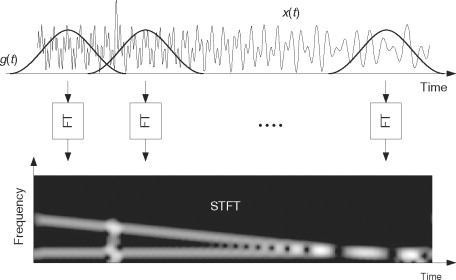
\includegraphics[height=5cm]{fig1.jpg}
    \centering
    \caption{Computing STFT ($g$ is the (sliding) window function)}
\end{figure}	

	Here, $\omega[n]$ is the window function, typically a Hann window or Gaussian window.
	(Window function is a function that is zero-valued outside some chosen interval, and usually symmetric.)

	
\subsection{Mel scale/Mel spectrogram}
	The Mel scale, introduced by Stevens, Volkmann, and Newman in 1937, is a perceptual scale of pitches judged by listeners to be equal in distance from one another.
	In other words, the Mel Scale is constructed such that sounds of equal distance from each other on the Mel Scale, also “sound” to humans as they are equal in distance from one another.	
	(Think of the Mel scale as a psychoacoustic scale)

	There isn't a "single" Mel scale formula, but the popular formula from O'Shaughnessy's book is as the following:
	$$m = 2595 \log_{10} \left( 1 + \frac{f}{700} \right)$$	
	Mel spectrogram is the combination of above concepts: spectrogram with Mel scale as its y-axis.


\subsection{Mel-frequency cepstrum (MFC)}

\begin{wrapfigure}{l}{6cm}
  \begin{center}
    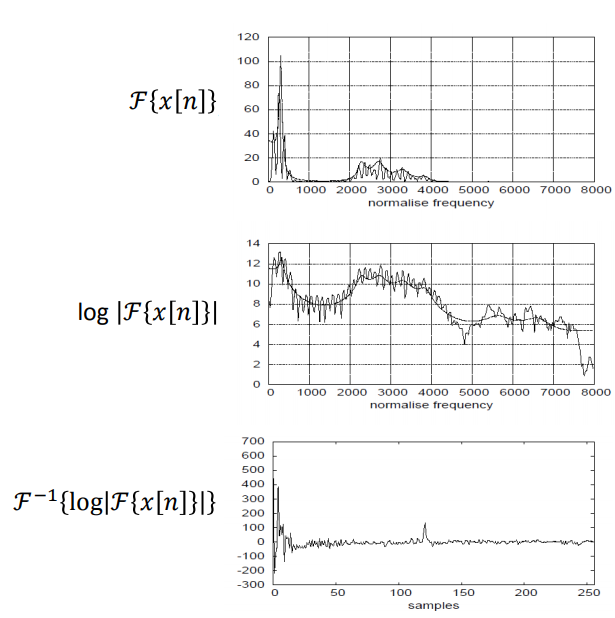
\includegraphics[height=5cm]{fig2.png}
  \end{center}
    \caption{Computing cepstrum}
\end{wrapfigure}

	The power cepstrum of a time signal $x[n]$, as defined by Bogert {\it et al.} in 1963, is 
	$$c[n] = \left| \mathcal{F}^{-1} \left\{ \log \left( |\mathcal{F} \{x[n]\}|^2 \right) \right\} \right|^2$$
	Intuitively, this gives us the information about the rate of change in the different spectrum bands.
	This is often utilized as a feature vector for representing musical signals.
	
	But in musical signals, the spectrum is usually first transformed using the Mel scale. The result is called the Mel-frequency cepstrum (MFC), and we call its coefficients as the Mel-frequency cepstral coefficients (MFCCs).
	In the MFC, the frequency bands are equally spaced on the Mel scale, which approximates the human auditory system's response more closely than the linearly-spaced frequency bands used in the normal cepstrum. This frequency warping can allow for better representation of sound, for example, in audio compression.
	
	MFCCs of $x[n]$ are commonly derived as follows (with some variantions in the process, depending on the task):
	\begin{enumerate}
		\item Take the Fourier transform of a windows excerpt of $x[n]$
		\item Map the powers of the obtained spectrum onto the Mel scale (using triangular overlapping windows)
		
		\item Take the logs of the powers at each of the mel frequencies
		
		\item Take the discrete cosine transform of the list of mel log powers
		
		\item The MFCCs are the amplitudes of the resulting spectrum
	\end{enumerate}


\begin{wrapfigure}{l}{5cm}
  \begin{center}
    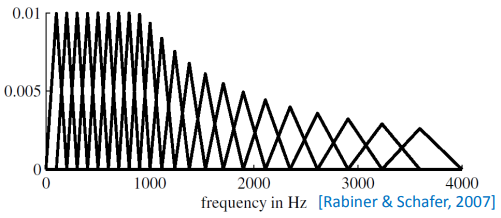
\includegraphics[height=2cm]{fig3.png}
  \end{center}
    \caption{$V_r[k]$}
\end{wrapfigure}

	Summarizing above using mathematical expressions:
	$$MFCC[m] = \frac{1}{R} \sum_{r = 1}^R \log (MF[r]) \cos \left[ \frac{2\pi}{R} \left(r + \frac{1}{2}\right)m \right]$$
	where
	$$MF[r] = \left( \sum_{k = L_r}^{U_r} \left| V_r[k] \right|^2 \right)^{-1} \sum_{k = L_r}^{U_r} \left| V_r[k] X(n, k) \right|$$
	\\
	($V_r[k]$ is the triangular weighting function for the $r$-th filter, ranging from DFT index $L_r$ to $U_r$. Usually, $MFCC[m]$ is evaluated for a number of coefficients $N_{MFCC}$ that is less than the number of mel-filters $R$)


\subsection{Spectral statistics}

\subsubsection{Spectral centroid}

Spectral centroid indicates where the "center of mass" of the mass of the spectrum is located {\it i.e.} it represents {\it at which frequency the energy of a spectrum is centered upon}.
$$f_c = \frac{\sum_k S(k) f(k)}{\sum_k S(k)}$$
where $S(k)$ is the spectral magnitude at frequency bin $k$, $f(k)$ is the frequency at bin $k$.

\subsubsection{(Octave-based) Spectral Contrast}

	MFCC is a representation of spectral characteristics of music that averages the spectra in each sub-band and reflects the average spectral characteristics. (It is sometimes called the average spectral envelope)
	But MFCC cannot represent the relative spectral characteristics in each sub-band, which might be more important in our music genre classification problem.

	Octave-based Spectral Contrast feature considers the strength of spectral peaks and spectral valleys in each sub-band separately to represent the relative spectral characteristics.
	For most music, the strong spectral spectral peaks roughly correspond with harmonic components; while non-harmonic components, or noises, often appear at spectral valleys.
	This is why the {\it Spectral Contract feature roughly reflects the relative distribution of harmonic and nonharmonic components in the spectrum}, while MFCC loses that information.

	To make this point more clear, consider two spectra with different spectral distribution and similar average spectral characteristics. Then, MFCC won't be able to distinguish between them while Spectral Contrast may perform better.

\begin{figure}[hbt!]
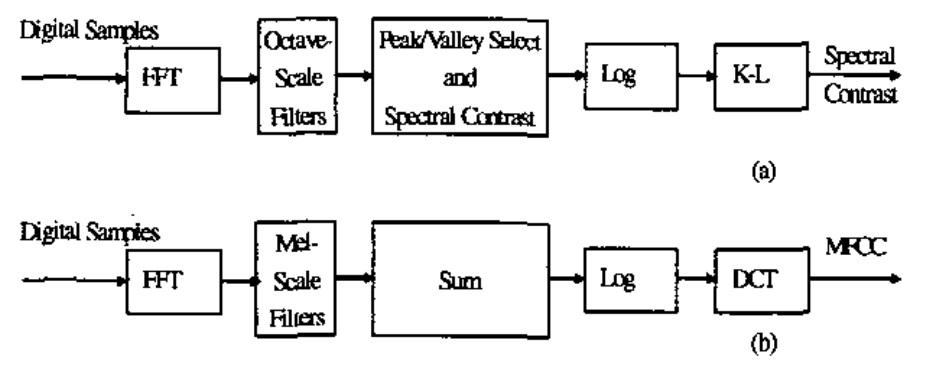
\includegraphics[height=4cm]{fig4.png}
    \centering
    \caption{Comparison of (a) Octave-based Spectral Contrast and (b) MFCC}
\end{figure}

Main differences between the Spectral Contrast and MFCC are...

\begin{itemize}
	\item The filter bank is different; Octave-based Spectral Contrast uses octave-scale filters while MFCC uses Mel-scale filters.
	(Although Mel-scale is suitable for general auditory model, octave-scale filter is more suitable for music processing.)
	
	\item Spectral Contrast extracts the spectral peaks, valleys, and their differences in each sub-band while MFCC sums the FFT amplitudes
	
	\item Spectral Contrast feature uses the Karhunen-Lo\'eve Transform (KLT) while MFCC uses a Discrete Cosine Transform (DCT).
\end{itemize}

To solve the problem of some relativity among the different dimensions of raw feature, the KLT is performed.
Then by the Karhunen-Lo\'eve Theorem, the feature vector is mapped into an orthogonal space, and the covariance matrix is diagonalized.
These properties of KLT make the classifying procedure easier and lead to good classification performance, even with simple classifier with Spectral Contrast (Jiang {\it et al.}).

\subsubsection{Chroma}
...?


\section{Method}

Please refer to our github repository\footnote{\url{https://github.com/iJinjin/CS470_Team23}} for the code.

\section{Contributions}

\begin{itemize}
\item Minsung Park: TBD

\item Youngjin Jin: Implementing the data processing code for the spectrogram and melspectrogram images, csv file generation, making the overall CNN architecture and code for training and testing CNN data, writing the README file, proof-checking the final report document

\item Junghyun Lee: TBD

\end{itemize}

\end{document}
